\chapter{How To}

This chapter provides a practical guide to generating and managing effect descriptions for the project, using scripts in the \texttt{bin/} directory. Some steps may seem tedious or complicated—editing multiple files, running scripts with specific arguments, or managing directory paths—but they are essential. With thousands and thousands of effects to handle, manual processing would be impractical; this automation ensures consistency, scalability, and differentiation of metadata, making it an extremely helpful approach for large-scale effect management.



\subsection{Add and Auto-Generate Effect Strings from Templates}

This section guides you through creating effect descriptions from templates using scripts in the \texttt{bin/} directory. You’ll combine placeholder values from \texttt{placeholders/} with templates from \texttt{effects/} to generate a list of effects.

\subsubsection{What You’ll Need}
\begin{itemize}
	\item A Unix-like system (e.g., Linux, macOS) with Bash and Python 3 installed or Windows with Cygwin and a compatible python setup.
	\item The project directory structure: \texttt{bin/}, \texttt{placeholders/}, and \texttt{effects/}. This should already exist if you cloned this project using \textit{git}.
\end{itemize}

\subsubsection{Step-by-Step Guide}

\paragraph{Step 1: Set Up Your Placeholders and Templates}
\begin{enumerate}
	\item Open \texttt{effects/all\_effect\_templates.txt} in a text editor.
	\item Add or edit effect templates using placeholders like \texttt{<number>} or \texttt{<type>}. For example:
\begin{lstlisting}
Draw <number> cards
Gain <number> <type> points
\end{lstlisting}
	\item Save the file.
\end{enumerate}

\paragraph{Step 2: Configure Placeholders}
\begin{enumerate}
	\item Go to the \texttt{placeholders/} directory.
	\item For each placeholder in your templates (e.g., \texttt{<number>}, \texttt{<type>}), create or edit a file named \texttt{<placeholder>.txt}. Examples:
	\begin{itemize}
		\item \texttt{number.txt}: Add one number per line (e.g., \texttt{1}, \texttt{2}, \texttt{3}).
		\item \texttt{type.txt}: Add one type per line (e.g., \texttt{fire}, \texttt{water}).
	\end{itemize}
	\item Save your changes. Keep it simple—just list the values, no comments or extra formatting.
	\item[!!] Note: The placeholders correspond to file(s) in the \texttt{placeholders/} folder. The names of the placeholder files should match the names of the placeholders exactly.
\end{enumerate}

\paragraph{Step 3: (Optional) Filter and Refine Effects}
\begin{enumerate}
	\item Open \texttt{placeholders/combinations\_to\_remove.txt}.
	\item List phrases you don’t want in your effects, one per line. For example:
\begin{lstlisting}
# Skip useless effects
Draw 0 cards
\end{lstlisting}
	\item Open \texttt{placeholders/phrase\_replacements.txt}.
	\item Add replacements in \texttt{old phrase: new phrase} format, like:
\begin{lstlisting}
# Fix grammar
Gain 1 points: Gain 1 point
\end{lstlisting}
	\item Save both files. Use \texttt{\#} for comments if you’d like. If you include comments, the comments must be on their own line(s).
\end{enumerate}

\paragraph{Step 4: Generate Effects}
\begin{enumerate}
	\item Navigate to the \texttt{bin/} directory in your terminal:
\begin{lstlisting}[style=terminalstyle]
cd bin
\end{lstlisting}
	\item Run the generation script:
\begin{lstlisting}[style=terminalstyle]
python3 create_effect_combinations.py -f ../effects/all_effect_templates.txt
\end{lstlisting}
	\item If you are using the default file paths for the effect templates, you can omit the actual file (as seen in the above command) as the script will default to it.
\begin{lstlisting}[style=terminalstyle]
python3 create_effect_combinations.py -f
\end{lstlisting}
	\item Check \texttt{../effects/all\_effects.txt} for your generated effects (e.g., ``Draw 1 cards'', ``Gain 2 fire points'').
\end{enumerate}

\paragraph{Step 5: (Optional) Automate with a Script}
\begin{enumerate}
	\item For a one-command solution, run:
\begin{lstlisting}[style=terminalstyle]
./generate_and_order_effects.sh
\end{lstlisting}
	\item This cleans up old files and generates effects automatically. It also performs other steps and processes outlined later.
	\item Find the results in \texttt{../effects/all\_effects.txt}.
\end{enumerate}

\subsubsection{Tips}
\begin{itemize}
	\item \textbf{Customize Output}: Tweak \texttt{all\_effect\_templates.txt} or placeholder files to change effects.
	\item \textbf{Fix Errors}: If a script fails, double-check that files exist and paths are correct (e.g., \texttt{../placeholders/number.txt}).
	\item \textbf{See Results}: Your effects land in \texttt{all\_effects.txt} as plain text.
\end{itemize}







\subsection{Adding Metadata to Effects and Automating the Process}

This section explains how to add metadata (e.g., categories like \texttt{UNIT} or \texttt{SPELL}) to your effect descriptions using the \texttt{add\_csv\_field.py} script and how to automate metadata addition for all effects with \texttt{generate\_and\_order\_effects.sh}. You’ll work with files in the \texttt{bin/} and \texttt{effects/} directories, building on the effects generated earlier.

\subsubsection{What You’ll Need}
\begin{itemize}
	\item A Unix-like system (e.g., Linux, macOS) with Bash and Python 3 installed, or Windows with Cygwin and a compatible Python setup.
	\item The project directory structure: \texttt{bin/}, \texttt{placeholders/}, and \texttt{effects/}, already set up from cloning this project with \textit{git}.
	\item An existing \texttt{all\_effects.txt} file in \texttt{effects/} from the previous section.
\end{itemize}

\subsubsection{Step-by-Step Guide}

\paragraph{Step 1: Add Metadata with \texttt{add\_csv\_field.py}}
\begin{enumerate}
	\item Navigate to the \texttt{bin/} directory in your terminal:
\begin{lstlisting}[style=terminalstyle]
cd bin
\end{lstlisting}
	\item Run \texttt{add\_csv\_field.py} to add a metadata column to your effects. For example, to mark effects as \texttt{UNIT}:
\begin{lstlisting}[style=terminalstyle]
python3 add_csv_field.py -i ../effects/all_effects.txt -o ../effects/effects_with_placeholders.csv -c UNIT -t "You can send up to <number> card"
\end{lstlisting}
	\item Explanation:
	\begin{itemize}
		\item \texttt{-i}: Input file (e.g., \texttt{all\_effects.txt}).
		\item \texttt{-o}: Output CSV file (e.g., \texttt{effects\_with\_placeholders.csv}).
		\item \texttt{-c}: Column name to add or to set to True (if it exists) (e.g., \texttt{UNIT}).
		\item \texttt{-t}: Pattern with placeholders to match (e.g., \texttt{You can send up to <number> card}).
	\end{itemize}
	\item Assuming all files are left in their default locations, this script can be used without an \textit{input} or \textit{output} arguments to get the same result
\begin{lstlisting}[style=terminalstyle]
python3 add_csv_field.py -c UNIT -t "You can send up to <number> card"
\end{lstlisting}
	\item Repeat for other categories. For example, to mark \texttt{SPELL} effects:
\begin{lstlisting}[style=terminalstyle]
python3 add_csv_field.py -c SPELL -t "Your opponent loses <number> point"
\end{lstlisting}
	\item Check \texttt{../effects/effects\_with\_placeholders.csv}. It will list effects with columns like \texttt{UNIT} and \texttt{SPELL}, set to ``True'' or ``False'' based on matches.
\end{enumerate}

\paragraph{Step 2: Understand How It Works}
\begin{enumerate}
	\item The script uses placeholder files from \texttt{../placeholders/} (e.g., \texttt{number.txt}, \texttt{type.txt}) to expand patterns. For example, ``Gain <number> <type> points'' matches ``Gain 1 fire points'' if \texttt{number.txt} has ``1'' and \texttt{type.txt} has ``fire''.
	\item You can use \texttt{-e} instead of \texttt{-t} for exact matches:
\begin{lstlisting}[style=terminalstyle]
python3 add_csv_field.py -c UNIT -e "Gain 1 fire point"
\end{lstlisting}
	\item[] \textit{Note}: Each run adds or updates one column. Use the output CSV as input for the next category to build up metadata.
\end{enumerate}

\paragraph{Step 3: Automate Metadata for All Effects}
\begin{enumerate}
	\item The \textit{generate\_and\_order\_effects.sh} script handles automating calls to \textit{create\_effect\_combinations.py } and \textit{add\_csv\_field.py} with the proper parameters to get the desired output metadata for all possible effects that are currently configured. This file has a lot of entries as well as some loops that specify similar entries with subtle differences for certain effects.
	\item Modify the automation script mentioned above appropriately for any effect additions to get the desired meta-data.
	\begin{itemize}
		\item To add an effect which should be appropriate for any level of spell, find the appropriate for loop within the file and add the line for the spell. For example:
\begin{lstlisting}[style=shellstyle]
# Spell effects that are the same for each level
for level in LEVEL_{1..3}; do
    python3 add_csv_field.py -c "$level" -m SPELL -t "Your opponent cannot play <types> cards next turn"
    ...
    // Add Desired additions here.
done
\end{lstlisting}
		\item To add an effect which should be appropriate for any specific number based on the level of spell, find the appropriate \textit{for} loop within the file and add the line for the spell. These are spells that contain a number placeholder which scales with the level of the card. A loop exists for both spells and units but is slightly different for each. For example:
\begin{lstlisting}[style=shellstyle]
# Some various <number> effect combinations for spells.
NUMS=(zero one two three four) # Array for number words
for l in "LEVEL_1 1 2" "LEVEL_2 2 3" "LEVEL_3 3 4"; do
	read level min max <<< "$l"
	for ((m=min; m<=max; m++)); do
		python3 add_csv_field.py -c "$level" -m SPELL -t "Reveal the top ${NUMS[m]} card$( ((m>1)) && echo "s") of your deck and play one <type> card from among them"
		...
		// Add Desired additions here.
	done
done
\end{lstlisting}
		\item To add an effect which should be appropriate for any specific rank based on the level of spell, find the appropriate \textit{for} loop within the file and add the line for the spell. These are spells that contain a rank placeholder which scales with the level of the card. A loop exists for both spells and units but is slightly different for each. For example:
\begin{lstlisting}[style=shellstyle]
# Some various <rank> effect combinations for spells.
for l in "LEVEL_1 1 2" "LEVEL_2 2 4" "LEVEL_3 4 5"; do
	read level min max <<< "$l"
	for ((m=min; m<=max; m++)); do
		python3 add_csv_field.py -c "$level" -m SPELL -t "Add up to <number> rank ${m} light cards from your deck to your hand."
		...
		// Add Desired additions here.
	done
done
\end{lstlisting}
	\item To add effects that are specific to a unit or spell, add a line with the specific unit/spell specifier as well as the effect string to search for in the appropriate section. For example:
	\begin{lstlisting}[style=shellstyle]
# Add some unit specific effects.
python3 add_csv_field.py -c UNIT -t "You can send up to <number> card"
...
// Add Desired additions here.
	\end{lstlisting}
	\item Exceptions to the above loops exist for specific effects that require specific levels which they should correspond to. These can be added in the appropriate exceptions section. For example:
\begin{lstlisting}[style=shellstyle]
# Exceptions to the below loop(s).
python3 add_csv_field.py -c LEVEL_1 -m SPELL -t "Destroy one <type> card on the field"
...
// Add Desired additions here.
\end{lstlisting}
\end{itemize}
	\item Run the automation script:
\begin{lstlisting}[style=terminalstyle]
./generate_and_order_effects.sh
\end{lstlisting}
	\item This script:
	\begin{itemize}
		\item Generates effects from \texttt{all\_effect\_templates.txt} (as in the previous section).
		\item Adds metadata columns (e.g., \texttt{UNIT}, \texttt{SPELL}) based on predefined patterns or exact matches.
		\item Cleans up old files and organizes the output.
	\end{itemize}
	\item Check \texttt{../effects/effects\_with\_placeholders.csv} for the final result, which includes all effects with metadata columns added automatically.
\end{enumerate}

\subsubsection{Tips}
\begin{itemize}
	\item \textbf{Customize Metadata}: Edit the patterns or exact strings in your \texttt{add\_csv\_field.py} commands to match your effects.
	\item \textbf{Fix Errors}: Ensure input files exist and placeholder files in \texttt{../placeholders/} match your patterns.
	\item \textbf{See Results}: Open \texttt{effects\_with\_placeholders.csv} in a spreadsheet or text editor to review metadata.
\end{itemize}

\subsubsection{What You Get}
\begin{itemize}
	\item \texttt{effects/effects\_with\_placeholders.csv}: A semicolon-delimited CSV with effects and metadata columns (e.g., \texttt{UNIT}, \texttt{SPELL}) set to ``True'' or ``False''.
	\item At the time of writing this, the meta-data columns programmed into this automation script(s) create columns for UNIT, SPELL, LEVEL\_1, \dots LEVEL\_5. This allows the distinction between the two main sets of cards (units and spells) as well as different effects that should/could be valid for the varying levels of those cards.
\end{itemize}
















\subsection{Generating Random Effect Pairs for Cards}

This section shows you how to use \texttt{generate\_random\_effects.py} to create specific pairs of effects for a card, such as for a trading card game. The script filters effects from a CSV based on metadata columns and generates random pairs from the filtered list, perfect for assigning unique effect combinations to a card.

\subsubsection{What You’ll Need}
\begin{itemize}
	\item Python 3 installed and the project structure (\texttt{bin/}, \texttt{effects/}) set up.
	\item \texttt{effects/effects\_with\_placeholders.csv} from previous sections, with metadata columns like \texttt{UNIT} or \texttt{SPELL}.
\end{itemize}

\subsubsection{Steps}
\begin{enumerate}
	\item Navigate to the \texttt{bin/} directory:
\begin{lstlisting}[style=terminalstyle]
cd bin
\end{lstlisting}
	\item Run the script to generate pairs for a card. For example, to get 10 random \texttt{UNIT} effect pairs:
\begin{lstlisting}[style=terminalstyle]
python3 generate_random_effects.py -c UNIT
\end{lstlisting}
	\item For multiple filters (e.g., \texttt{UNIT} and \texttt{LEVEL\_1}), use:
\begin{lstlisting}[style=terminalstyle]
python3 generate_random_effects.py -c UNIT -c LEVEL_1
\end{lstlisting}
	\item To change the number of pairs (e.g., 5 instead of 10):
\begin{lstlisting}[style=terminalstyle]
python3 generate_random_effects.py -c UNIT -p 5
\end{lstlisting}
	\item The script defaults to \texttt{../effects/effects\_with\_placeholders.csv}. For a custom file, add it:
\begin{lstlisting}[style=terminalstyle]
python3 generate_random_effects.py my_effects.csv -c UNIT
\end{lstlisting}
	\item Check the terminal output for numbered pairs of effects from the first column (e.g., ``Gain 1 fire points'' paired with ``Draw 2 cards'').
\end{enumerate}

\subsubsection{Tips}
\begin{itemize}
	\item Use metadata columns added earlier (e.g., \texttt{UNIT}, \texttt{SPELL}) to filter effects specific to your card.
	\item If no pairs appear, ensure your CSV has enough ``True'' rows for the specified columns.
\end{itemize}














\subsection{Creating a TTCG Trading Card}

This section explains how to use \texttt{create\_card.py} to generate a trading card image for the TTCG format, complete with effects, stats, and a custom design. It builds on effects generated earlier, turning them into a visual card.

\subsubsection{What You’ll Need}
\begin{itemize}
	\item Python 3 with the \texttt{Pillow} library installed (\texttt{pip install Pillow}).
	\item The project structure (\texttt{bin/}, \texttt{images/}) set up, with type images (e.g., \texttt{fire.png}) in \texttt{../images/card pngs/}.
\end{itemize}

\subsubsection{Steps}
\begin{enumerate}
	\item Navigate to the \texttt{bin/} directory:
\begin{lstlisting}[style=terminalstyle]
cd bin
\end{lstlisting}
	\item Run the script to create a card. For example:
\begin{lstlisting}[style=terminalstyle]
python3 create_card.py --name "Fire Dragon" --type fire --level 3 --subtype Dragon Spirit --effect1 "Gain 2 fire points" --effect2 "Draw 1 cards"
\end{lstlisting}
	\item Customize further if desired:
	\begin{itemize}
		\item Add stats: \texttt{--attack 1000 --defense 500}.
		\item Use a custom image: \texttt{--image ../images/custom.png}.
		\item Set output folder: \texttt{-o ../my\_cards}.
	\end{itemize}
	\item Check the output folder (defaults to \texttt{../images/generated\_cards/}) for the card, e.g., \texttt{ttcg\_card\_Fire\_Dragon.png}. It’s a 750x1050 pixel image with your card details.
\end{enumerate}

\subsubsection{Example}
Below is an example command (without an image specified) with the matching output seen in Figure \ref{fig:sample_generated_output}.
\begin{lstlisting}[style=terminalstyle]
./create_card.py --name "This is an even longer name for testing long names" --level 3 --effect1 "This is some sample text to represent an effect on the card." --effect2 "This is some sample text to represent an effect on the card. It's quite long to test longer effects. That way I can ensure the text fits nicely."
\end{lstlisting}

\begin{figure}[h]
	\centering
	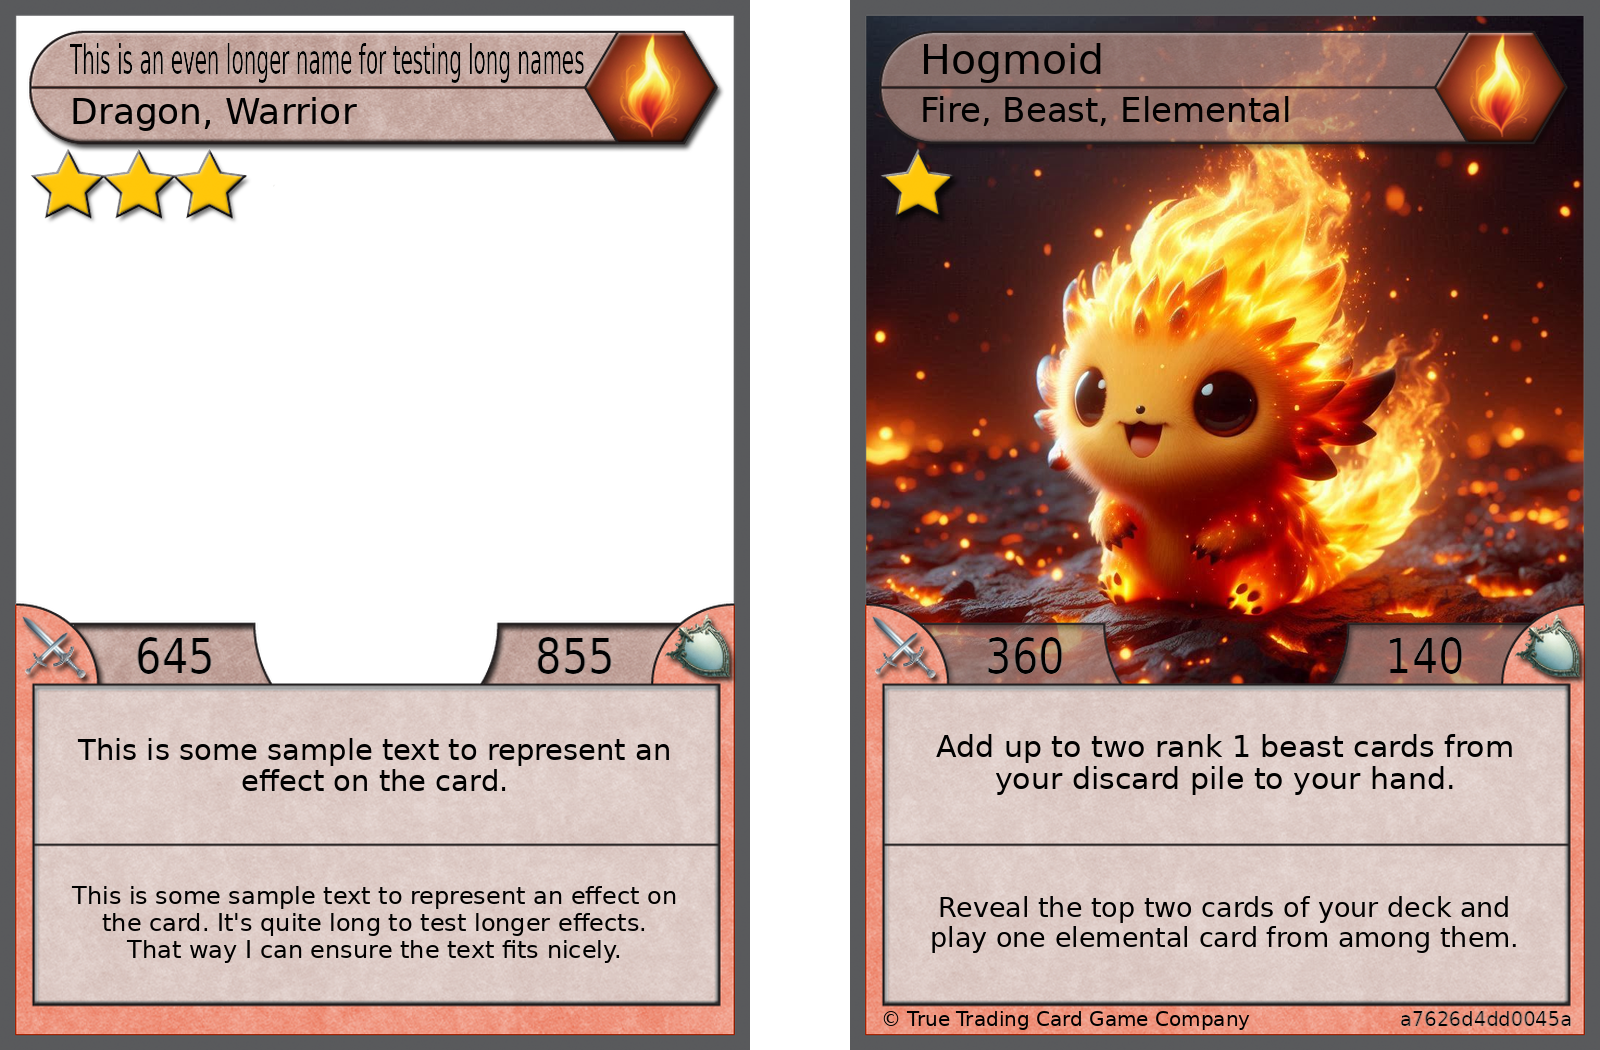
\includegraphics[width=0.4\textwidth]{images/sample_generated_output.png} 
	\caption{This is a sample card with a fake name, subtypes, and some dummy text in the effect slots. This is to demonstrate the output of the \textit{create\_card.py} script.}
	\label{fig:sample_generated_output}
\end{figure}

\subsubsection{Tips}
\begin{itemize}
	\item Use effects from \texttt{all\_effects.txt} or pairs from \texttt{generate\_random\_effects.py}.
	\item If stats are omitted, they’re random but scaled to level (total = level * 500).
	\item Ensure type images (e.g., \texttt{fire.png}) exist in \texttt{../images/card pngs/}, or it falls back to a default.
	\item Use \texttt{-o} to save cards elsewhere; ensure the folder exists or the script may fail.
\end{itemize}










\subsection{Creating TTCG Trading Card(s) With The UI}

This section provides a step-by-step guide to creating trading cards using the TTCG Card Creator graphical user interface (GUI). The UI allows you to input card details, preview the card, and save it to a CSV file while ensuring unique card names. The interface features a dark theme for comfortable use, with all fields and previews clearly visible.

\subsubsection{Launching the Application}

\begin{enumerate}
    \item Ensure you have Python 3 installed, along with required libraries: \texttt{tkinter}, \texttt{PIL} (Pillow), and \texttt{csv}. Install them using:
\begin{lstlisting}[style=terminalstyle]
pip install pillow
\end{lstlisting}
    \item Place your card images in a directory structure (e.g., \texttt{../images/units/fire/}, \texttt{../images/units/light/}, etc.), organized by type if desired.
    \item Run the script from the command line:
\begin{lstlisting}[style=terminalstyle]
python3 card_maker_ui.py
\end{lstlisting}
          \begin{itemize}
              \item \texttt{-i}: Path to the effects CSV file (defaults to \texttt{effects/effects\_with\_placeholders.csv}).
              \item \texttt{-o}: Path to the output card list CSV (defaults to \texttt{card\_list/card\_list.csv}).
          \end{itemize}
    \item The GUI will open displaying three main sections: Card Details (left), Card Preview (middle), and Effects Generator (right).
\end{enumerate}

\begin{figure}[h]
	\centering
	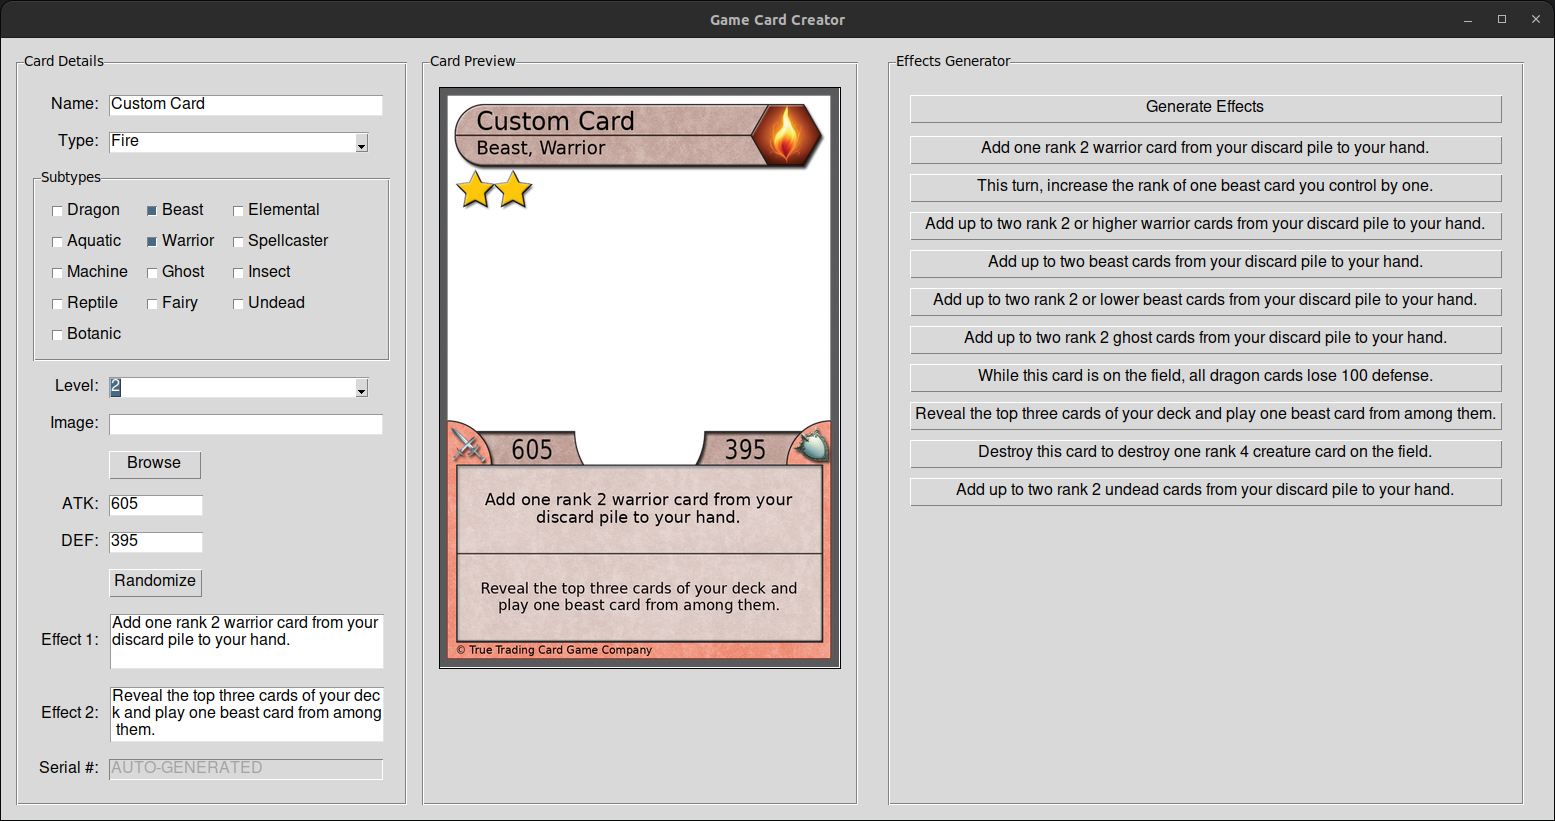
\includegraphics[width=\textwidth]{images/ui_sample.png} 
	\caption{This is a sample display of the \texttt{card\_maker\_ui.py}}
	\label{fig:sample_ui_window}
\end{figure}

\subsubsection{Creating a Card}

\begin{enumerate}
    \item \textbf{Set the Image:}
          \begin{itemize}
              \item In the \texttt{Card Details} section, click the \texttt{Browse} button below the \texttt{Image} field to select an image file (e.g., \texttt{Ember Foxling.jpg}).
              \item The image path will populate the entry field, and the card name will update to the filename (e.g., \texttt{Ember Foxling}) if the current name is \texttt{Unnamed}.
              \item The type (e.g., \texttt{Fire}) will automatically set if it’s in the image path and matches a predefined type list.
              \item Use \texttt{Next Image} to cycle to the next image in the folder, skipping any whose names are already in \texttt{card\_list/card\_list.csv}.
              \item Use \texttt{Flip Image} to horizontally flip the selected image if needed.
          \end{itemize}

    \item \textbf{Enter Card Details:}
          \begin{itemize}
              \item \texttt{Name}: Edit the auto-filled name (e.g., change \texttt{Ember Foxling} to \texttt{Ember Foxling Alpha}) if desired.
              \item \texttt{Type}: Select from the dropdown (e.g., \texttt{Fire}, \texttt{Water}) or keep the auto-detected type.
              \item \texttt{Subtypes}: Check boxes for applicable subtypes (e.g., \texttt{Beast}, \texttt{Elemental}). For \texttt{Spell} cards, subtypes are cleared automatically.
              \item \texttt{Level}: Choose a level (1--5) from the dropdown.
              \item \texttt{ATK} and \texttt{DEF}: Enter attack and defense values manually (e.g., \texttt{360} and \texttt{140}), or click \texttt{Randomize} to generate values based on the level.
          \end{itemize}

    \item \textbf{Add Effects:}
          \begin{itemize}
              \item In the \texttt{Effects Generator} section, click \texttt{Generate Effects} to populate 18 buttons with effect suggestions from \texttt{effects/effects\_with\_placeholders.csv}.
              \item Click an effect button to assign it to \texttt{Effect 1} or \texttt{Effect 2} (e.g., \texttt{Add up to two rank 1 beast cards from your discard pile to your hand}).
              \item Manually edit \texttt{Effect 1} and \texttt{Effect 2} text boxes if needed.
          \end{itemize}

    \item \textbf{Adjust Transparency:}
          \begin{itemize}
              \item In the \texttt{Card Preview} section, select a transparency level (50\%, 60\%, 75\%, or 100\%) using the checkboxes. The preview updates instantly.
          \end{itemize}

    \item \textbf{Preview the Card:}
          \begin{itemize}
              \item The \texttt{Card Preview} canvas (middle section) displays the card with the selected image, details, and effects. It updates automatically as you change fields.
          \end{itemize}

    \item \textbf{Save the Card:}
          \begin{itemize}
              \item Click \texttt{Save to Card List} in the \texttt{Card Preview} section.
              \item The card is saved to \texttt{card\_list/card\_list.csv} with a unique serial number (auto-generated) if:
                    \begin{itemize}
                        \item The name isn’t already in the CSV.
                        \item The exact card data (all fields) isn’t a duplicate.
                        \item The effect combination isn’t already used.
                    \end{itemize}
              \item If saved, the UI loads the next image with a unique name. If skipped (e.g., duplicate name), it still advances to the next image.
              \item Check the console or log for messages like \texttt{Card data saved} or \texttt{Card already exists}.
              \item The save feature does not generate the output card, but rather saves all of the various card data to the \texttt{card\_list/card\_list.csv} file for them to be generated later.
          \end{itemize}

    \item \textbf{Reset the UI:}
          \begin{itemize}
              \item Click \texttt{Reset} to clear all fields and start over.
          \end{itemize}
          
	\item \textbf{Generate the card Image File(s):}
	    \begin{itemize}
	        \item Once the \texttt{card\_list/card\_list.csv} is populated with the desired card values, the \textit{create\_card.py} script can be used to generate the card art for each card.
	        \item Run the \textit{create\_card.py} script with the spreadsheet option pointing to the \texttt{card\_list/card\_list.csv}.
\begin{lstlisting}[style=terminalstyle]
python3 create_card.py -S card_list/card_list.csv
\end{lstlisting}
			\item The card images will output to the \texttt{../images/generated\_cards} folder.
	    \end{itemize}
\end{enumerate}

\subsubsection{Understanding the Output}

\begin{itemize}
    \item Cards are saved to \texttt{card\_list/card\_list.csv} in the format:
\begin{lstlisting}
NAME;TYPE;SUBTYPES;LEVEL;IMAGE;ATTACK;DEFENSE;EFFECT1;EFFECT2;SERIAL;RARITY;TRANSPARENCY
Ember Foxling;Fire;Beast;1;../images/units/fire/Ember Foxling.jpg;360;140;...;...;a7626d4dd0045a;0;50
\end{lstlisting}
    \item The \texttt{IMAGE} field uses a relative path from the script directory.
    \item \texttt{RARITY} defaults to 0 (not editable in the UI yet).
\end{itemize}

\subsubsection{Tips and Troubleshooting}

\begin{itemize}
    \item \textbf{Duplicate Names:} If a name exists in \texttt{card\_list/card\_list.csv}, the UI skips to the next image. Ensure image filenames are unique or edit the name manually.
    \item \textbf{Image Not Loading:} Verify the image path is correct and the file exists. Check console logs for \texttt{Invalid image path} errors.
    \item \textbf{Effects Not Generating:} Ensure \texttt{effects\_with\_placeholders.csv} exists and contains valid effect templates.
    \item \textbf{UI Not Responding:} Check for errors in the console and ensure all dependencies are installed.
\end{itemize}

This interface streamlines card creation for TTCG, combining manual input with automated features like image cycling and effect generation. Experiment with different combinations to build your card collection!
